% document
\documentclass[11pt, aspectratio=169, final]{beamer}
\usepackage{adjustbox}
\adjustboxset*{center}
\usepackage{color}
\usepackage{xcolor}
\usepackage{textpos}

\usepackage{amsmath,amsfonts,amsthm} % Math packages
% theme coercion
\usetheme[width=2cm]{Hannover}
\usecolortheme{beaver}
\definecolor{base03}{HTML}{002B36}
\definecolor{base02}{HTML}{073642}
\definecolor{base01}{HTML}{586E75}
\definecolor{base3}{HTML}{FDF6E3}
\definecolor{solarblue}{HTML}{268bd2}
\definecolor{solarmagenta}{HTML}{D33682}
\setbeamercolor*{palette primary}{fg=darkred!60!black, bg=base01}  % title background
\setbeamercolor*{sidebar}{fg=darkred, bg=base03}
\setbeamercolor{frametitle}{bg=base01, fg=base3}
\setbeamercolor{title}{fg=base3}
\setbeamercolor{palette sidebar primary}{fg=base3}  % sidebar subsection
\setbeamercolor{palette sidebar secondary}{fg=base3}  % sidebar section
\setbeamercolor{palette sidebar tertiary}{fg=base3}  % sidebar name
\setbeamercolor{palette sidebar quaternary}{fg=base3}  % sidebar title
\setbeamercolor*{item}{fg=base01}
\setbeamertemplate{itemize items}[default]
\setbeamercovered{transparent}
\setbeamertemplate{navigation symbols}{}

% text
\usepackage[utf8]{inputenc}
\usepackage[T1]{fontenc}
\usepackage{enumerate}
\usepackage{soul}
\sethlcolor{yellow}
\renewcommand<>{\hl}[1]{\only#2{\beameroriginal{\hl}}{#1}}

% code
%\usepackage{minted}
%\definecolor{bg}{rgb}{0.95,0.95,0.95}
%\newminted{python}{fontsize=\scriptsize, numbersep=8pt,	gobble=0, frame=none, bgcolor=bg,	framesep=2mm, frame=leftline}

% quotes
\usepackage[T1]{fontenc}
\usepackage{libertine}
\usepackage{framed}
\newcommand*\openquote{\makebox(25,-22){\scalebox{5}{``}}}
\newcommand*\closequote{\makebox(25,-22){\scalebox{5}{''}}}
\colorlet{shadecolor}{base3}
\makeatletter
\newif\if@right
\def\shadequote{\@righttrue\shadequote@i}
\def\shadequote@i{\begin{snugshade}}
		\def\endshadequote{%
			\if@right\hfill\fi\end{snugshade}}
\@namedef{shadequote*}{\@rightfalse\shadequote@i}
\@namedef{endshadequote*}{\endshadequote}
\makeatother

% graphics
\usepackage{graphicx}
\usepackage{animate}
\usepackage{xmpmulti}

% bibliography
\usepackage[backend=bibtex,bibstyle=numeric,sorting=none]{biblatex}
\bibliography{bib}
\renewcommand\footnoterule{{\color{black} \hrule height 0pt}} % no line above footnotes
\renewcommand{\footnotesize}{\tiny}
\setbeamercolor{bibliography entry author}{fg=black,bg=black}
\setbeamercolor{bibliography entry title}{fg=black,bg=black}
\setbeamercolor{bibliography entry location}{fg=black,bg=black}
\setbeamercolor{bibliography entry note}{fg=black,bg=black}

% http://tex.stackexchange.com/questions/41683/why-is-it-that-coloring-in-soul-in-beamer-is-not-visible
\makeatletter
\newcommand\SoulColor{%
	\let\set@color\beamerorig@set@color
	\let\reset@color\beamerorig@reset@color}
\makeatother
\SoulColor

% logo (not built-in to hannover)
\addtobeamertemplate{headline}{}{%
\begin{textblock*}{\paperwidth}(0.5cm,\textheight-1.75cm)
	
\includegraphics[width=1cm]{logo} % logo of my university
\end{textblock*}}

\title{\textbf{WrightSim}}
\author{Kyle Sunden}
%\subtitle{}

\institute{University of Wisconsin--Madison}
\date{\today}
%\subject{}

\begin{document}
\maketitle

\section{Goals}

\begin{frame}{\textbf{Goals}}
\begin{itemize}
\item Reproduce experimental spectra \textit{in silico}.
\item Designed with experimentalists in mind.
\item Uses numerical integration for flexibility, accuracy and interpretability.
\item Focus on Frequency-domain spectroscopy, but techniques in principle extend to time-domain.
\item Output retains frequency and phase information, can be combined with other simulations and measured similar to a monochromator.
\item Selectivity in what portions of the overall signal are simulated, providing deeper understanding.
\end{itemize}
\end{frame}

\begin{frame}{\textbf{Sample Spectrum}}
\begin{center}
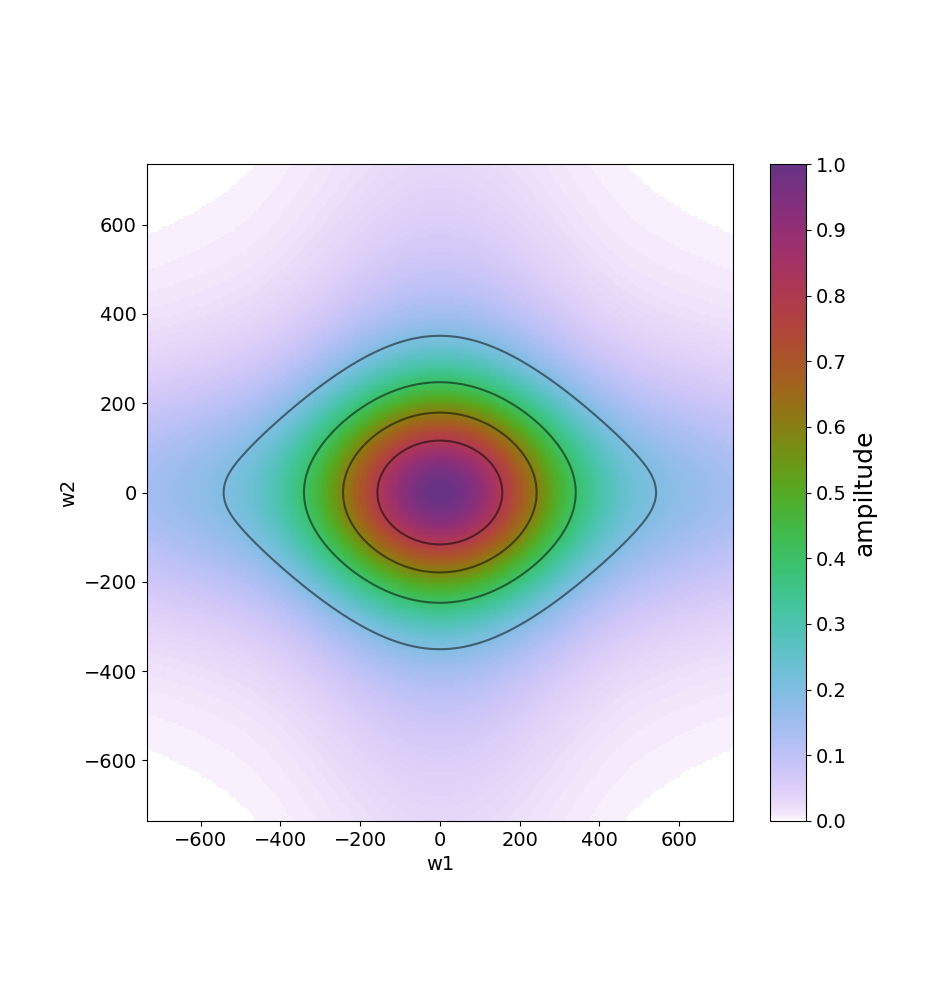
\includegraphics[height=0.8\textheight]{example_spectrum}
\end{center}
\end{frame}


\section{Theory}

\begin{frame}{\textbf{Introduction}}

Presented here is a description of \textit{what} is done to perform these simulations, to understand \textit{why} it works, please refer to Kohler, Thompson, and Wright\cite{Kohler_2017}.

The simulation uses a set number of electric fields (3, in the case of the simulation presented here).

These electric fields interact in combinatorially large different fashions.

Interactions create superposition coherences and/or populations in material systems.

\end{frame}

\begin{frame}{\textbf{Pathways}}
\begin{columns}
\column{0.5\textwidth}
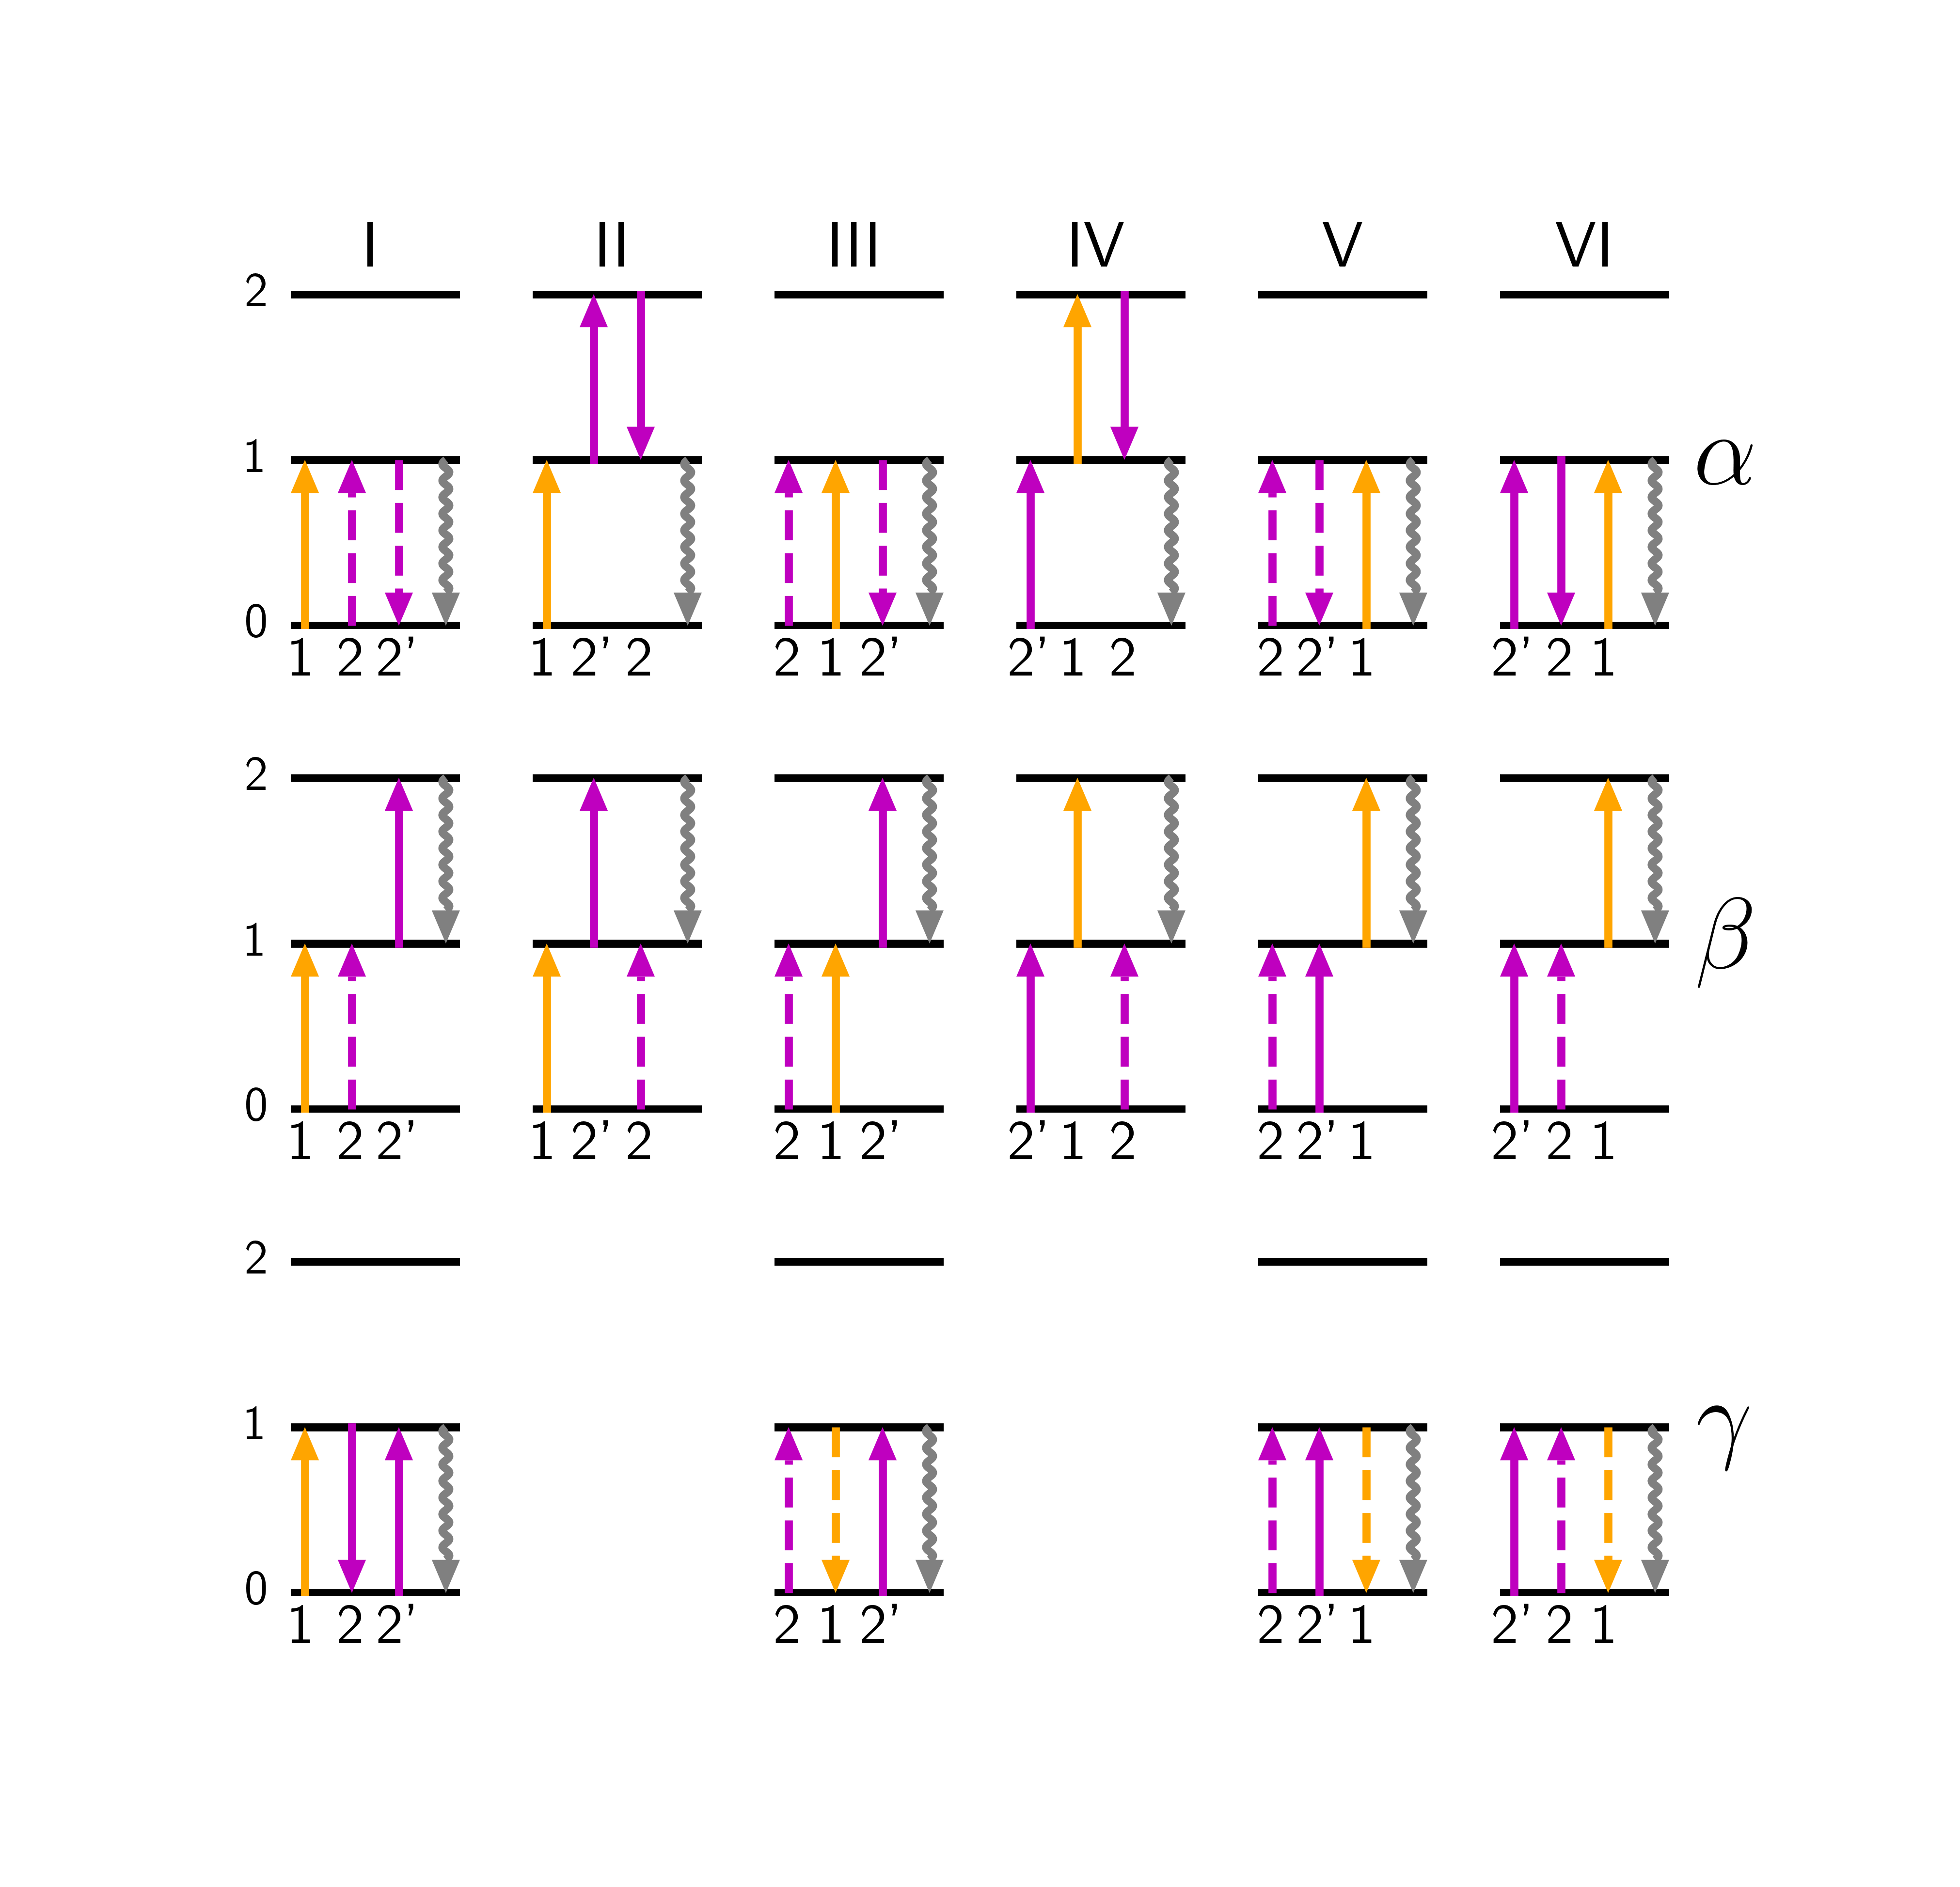
\includegraphics[height=0.8\textheight]{WMELs}
\column{0.5\textwidth}
There are six time orderings for interactions to occur (I-VI).

There are 16 independent pathways possible for two positive (solid up/dashed down) and one negative (dashed up/solid down) interactions.

Originally from \cite{Kohler_2017}.
\end{columns}
\end{frame}

\begin{frame}{\textbf{Finite state automaton}}
\begin{columns}
\column{0.8\textwidth}
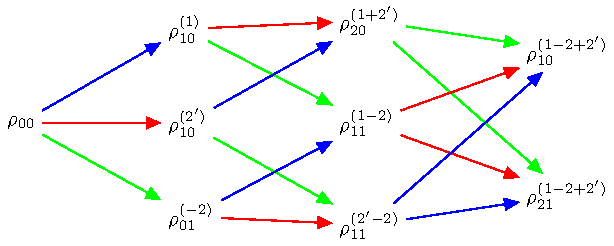
\includegraphics[width=\textwidth]{Matrix_Flow_Diagram}
Density elements, encoded with quantum state (subscript) and the electric fields which have interacted (superscript). Colored arrows represent the different electric fields.
All possible states which have the desired conditions for the process simulated are included.
These form the state vector (right).\cite{Kohler_2017}
\column{0.2\textwidth}
\begin{math}
\overline{\rho} \equiv
\begin{bmatrix}
\tilde{\rho}_{00} \\
\tilde{\rho}_{01}^{{-2}} \\
\tilde{\rho}_{10}^{{2^\prime}} \\
\tilde{\rho}_{10}^{{1}} \\
\tilde{\rho}_{20}^{{1+2^\prime}} \\
\tilde{\rho}_{11}^{{1-2}} \\
\tilde{\rho}_{11}^{{2^\prime-2}} \\
\tilde{\rho}_{10}^{{1-2+2^\prime}} \\
\tilde{\rho}_{21}^{{1-2+2^\prime}}
\end{bmatrix}
\end{math}
\end{columns}
\end{frame}

%\begin{frame}{\textbf{Hamiltonian Variables}}
%\begin{eqnarray}
%A_1 &\equiv& \frag{i} {2} \mu_{10}e^{-i\omega_1\tau_1)c_1(t-\tau_1)e^{i(\omega_1-\omega_{10})t} \\
%A_2 &\equiv& \frag{i} {2} \mu_{10}e^{-i\omega_2\tau_2)c_2(t-\tau_2)e^{i(\omega_2-\omega_{10})t} \\
%A_{2^\prime} &\equiv& \frag{i} {2} \mu_{10}e^{-i\omega_{2^\prime}\tau_{2^\prime})c_{2^\prime}(t-\tau_{2^\prime})e^{i(\omega_{2^\prime}-\omega_{10})t} \\
%B_1 &\equiv& \frag{i} {2} \mu_{21}e^{-i\omega_1\tau_1)c_1(t-\tau_1)e^{i(\omega_1-\omega_{21})t} \\
%B_2 &\equiv& \frag{i} {2} \mu_{21}e^{-i\omega_2\tau_2)c_2(t-\tau_2)e^{i(\omega_2-\omega_{21})t} \\
%B_{2^\prime} &\equiv& \frag{i} {2} \mu_{21}e^{-i\omega_{2^\prime}\tau_{2^\prime})c_1(t-\tau_{2^\prime})e^{i(\omega_{2^\prime}-\omega_{21})t}
%\end{eqnarray}

%\end{frame}

\begin{frame}{\textbf{Hamiltonian Matrix}}
\begin{math}
\overline{\overline{Q}} \equiv
\begin{bmatrix}
	0 & 0 & 0 & 0 & 0 & 0 & 0 & 0 & 0 \\
	-A_2 & -\Gamma_{10} & 0 & 0 & 0 & 0 & 0 & 0 & 0 \\
	A_{2^\prime} & 0 & -\Gamma_{10} & 0 & 0 & 0 & 0 & 0 & 0 \\
	A_1 & 0 & 0 & -\Gamma_{10} & 0 & 0 & 0 & 0 & 0 \\
	0 & 0 & B_1 & B_{2^\prime} & -\Gamma_{20} & 0 & 0 & 0 & 0 \\
	0 & A_1 & 0 & -A_2 & 0 & -\Gamma_{11} & 0 & 0 & 0 \\
	0 & A_{2^\prime} & -A_2 & 0 & 0 & 0 & -\Gamma_{11} & 0 & 0 \\
	0 & 0 & 0 & 0 & B_2 & -2A_{2^\prime} & -2A_1 & -\Gamma_{10} & 0 \\
	0 & 0 & 0 & 0 & -A_2 & B_{2^\prime} & B_1 & 0 & -\Gamma_{21}
\end{bmatrix}
\end{math}

Defines the transition between states, dependant on the electric field.
$\Gamma$ represents the dephasing/population decay.
$A$ and $B$ variables incorporate the dipole moment and electric field terms.\cite{Kohler_2017}

The dot product of this matrix and the density vector, $\overline{\rho}$, gives the change in in the density vector.
This is repeated over many small time periods to achieve the recorded results.
\end{frame}


\section{\texttt{NISE}}

\begin{frame}{\texttt{NISE}}
\texttt{NISE} (Numerical Integration of the Schr{\"o}dinger Equation) is an existing open-source implementation of the simulation for these kinds of spectra.\cite{nise}

It was written by Kohler and Thompson while preparing their manuscript.\cite{Kohler_2017}

\texttt{NISE} uses a slight variation on the algorithm presented, which allows for a 7-element state vector, but requires two simulations.

The end result is the same.


\texttt{NISE} is included as a reference for prior implementations.
\end{frame}

\section{\textbf{Algorithmic Improvements}}

\begin{frame}{\textbf{Algorithmic Improvements}}
\begin{itemize}

\item Use single 9 x 9 matrix rather than two 7 x 7 matrices.
\item $99.5\%$ of time is spent in highly parallelizable loop.
\item $1/3$ of time is spent in a single function, \texttt{ix\_}.
    \begin{itemize}
    \item Removed entirely, in favor of a simpler communication of what to record.
    \end{itemize}
\item Significant time in \texttt{rotor} function which computes $cos(\theta) + i*sin(\theta)$.
    \begin{itemize}
    \item Replaced with $exp(i*\theta)$, equivalent, more efficient, removed function call.
    \end{itemize}
\item Use variables to store and reuse redundant computations.
\end{itemize}

Resulted in almost an order of magnitude speed-up from algorithmic improvements alone.
Remained highly parallelizable.
\end{frame}

\begin{frame}{\textbf{Profile trace of \texttt{NISE}}}
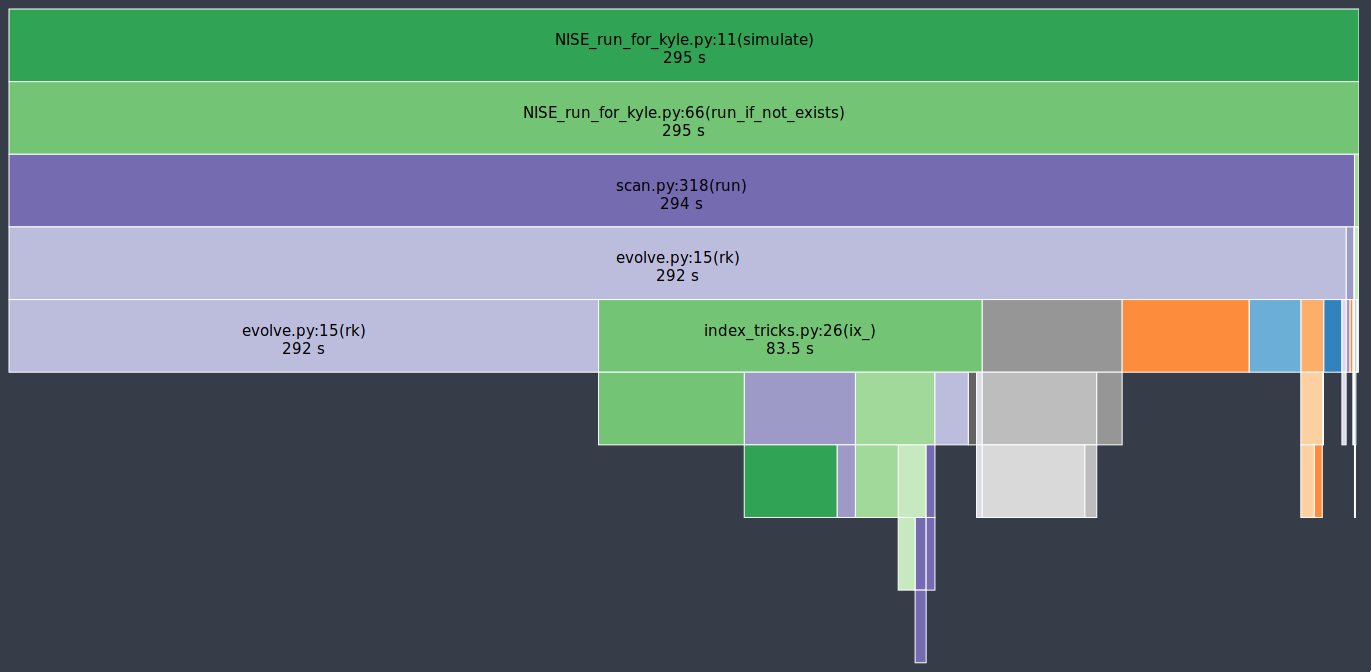
\includegraphics[width=0.9\textwidth]{NISE_prof}

Python \texttt{cProfile} trace, Single Core implementation, visualized with SnakeViz.\cite{snakeviz}
\end{frame}

\begin{frame}{\textbf{Profile trace of \texttt{WrightSim}}}
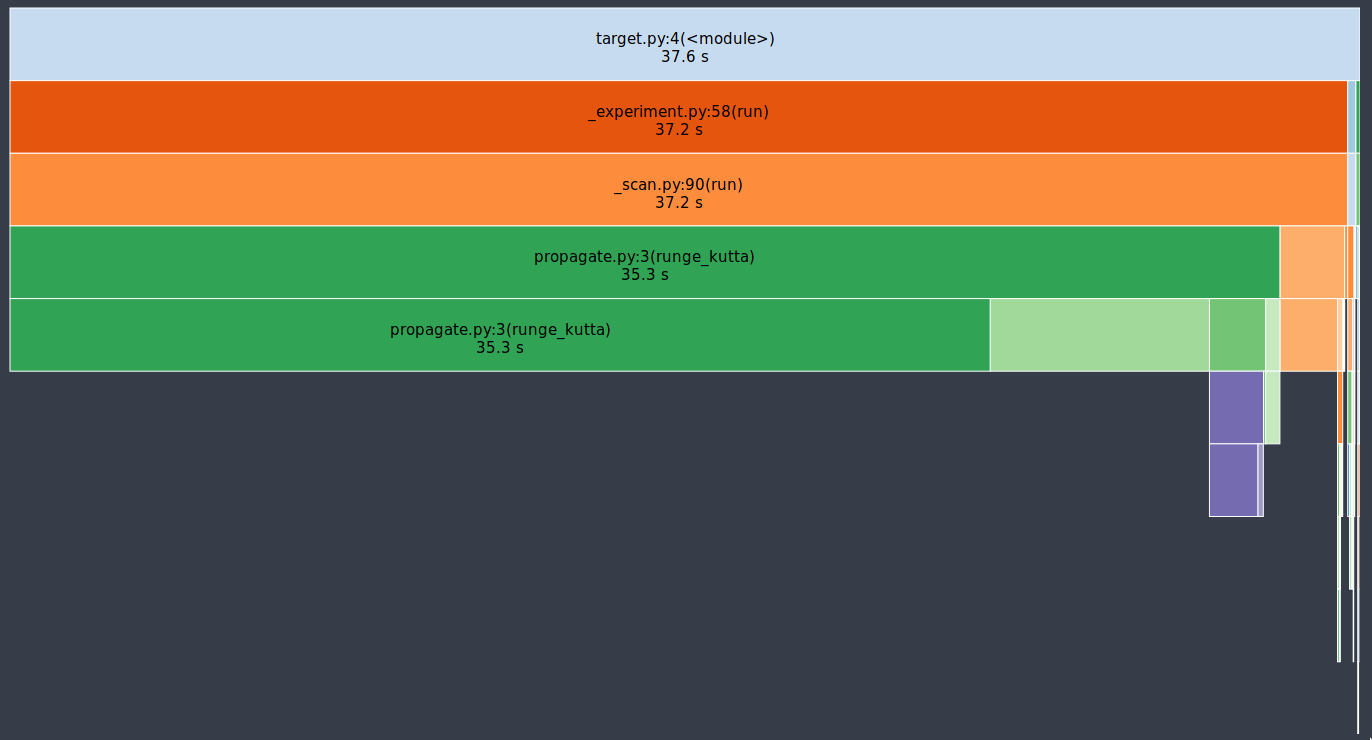
\includegraphics[width=0.9\textwidth]{WrightSim_prof}

Python \texttt{cProfile} trace, Single Core implementation, visualized with SnakeViz.\cite{snakeviz}
\end{frame}

\section{\textbf{Parallel Implementations}}

\begin{frame}{\textbf{Parallel Implementations}}
\begin{itemize}
\item \texttt{NISE} already had CPU multiprocessed parallelism, using Python standard library interfaces.
    \begin{itemize}
    \item \texttt{WrightSim} inherited this CPU parallel implementation
    \item Results in a 4x speed-up on a 4-core machine, almost no reduction due to Amdahl's law.
    \end{itemize}

\item A new Nvidia CUDA \cite{Nickolls_2008} implementation.
    \begin{itemize}
    \item Uses \texttt{PyCUDA} to call the kernel from within Python.
    \item Just-in-time compiled (using nvcc) from C source code stored in Python strings.
    \item Implementation differs slightly from pure Python implementation.
        \begin{itemize}
        \item Only actively used Hamiltonians are held in memory, Python implementation computes all time steps ahead of time.
        \item Similarly, only the actively used electric fields are held in memory.
        \item Hand written dot product and vector addition, rather than the numpy implementations.
        \end{itemize}

    \end{itemize}


\end{itemize}

\end{frame}

\subsection{Scaling Analysis}
\begin{frame}{\textbf{Scaling Analysis}}
\begin{center}
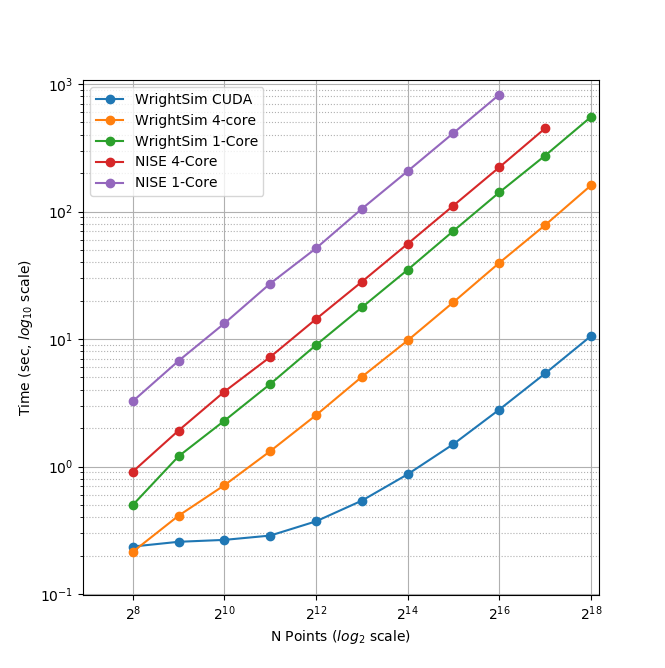
\includegraphics[height=0.8\textheight]{Scaling}
\end{center}
\end{frame}

\subsection{Limitations}

\begin{frame}{\textbf{Limitations}}
\begin{itemize}
\item For low number of points, the CUDA implementation is of limited use.
    \begin{itemize}
    \item Around 200 ms required for compilation.
    \item 4-Core multiprocessed becomes faster below approximately 256 points.
    \item CUDA implementation currently uses a hard coded block size of 256.
    \item Only multiples of 256 may be used at present to avoid illegal memory access.
    \end{itemize}


\item Independent CUDA simulations are memory limited.
    \begin{itemize}
    \item only a certain amount of memory can be allocated for a single CUDA process.
    \item Each point in the simulation requires 500 complex numbers (represented as doubles) to be allocated
    \item Additional data is needed, but dominated by this array.
    \item This array must be transferred back to the host.
    \item The limit is between $2^{18}$ and $2^{19}$ points
    \end{itemize}
\end{itemize}
\end{frame}


\section{\textbf{Future Work}}

\subsection{Features}
\begin{frame}{\textbf{Features}}
\begin{itemize}
\item Nonidealities like chirped pulses.
\item Inhomogeneous samples
    \begin{itemize}
    \item Results in broader peaks.
    \item Can be modelled by translating a single computed response and adding.
    \end{itemize}
\item Measuring signal using Fourier transforms similar to how a monochromator selects a signal.
\item Saving intermediate response values (Using HDF5 based file format)
\item Saving compiled CUDA binary for more than one run at a time
\end{itemize}
\end{frame}
\begin{frame}{\textbf{Metaprogramming Features}}
Metaprogramming techniques are those which modify the code that is run as the program executes.

Just-in-time compilation enables many opportunities for metaprogramming.
\begin{itemize}
\item Using same-named functions to change the exact algorithms, while other calling functions do not need to be edited.
\item Resolving shortcuts taken for statically allocated arrays.
\item Potentially, entire C functions could be dynamically generated by inspecting the Python code, resulting in new Hamiltonians only being required to be implemented once, in Python.
\end{itemize}
\end{frame}

\subsection{Usability}
\begin{frame}{\textbf{Usability}}
One important thing to do is to take a step back and think about how users interact with the program.
\begin{itemize}
\item Ensure the API is sensible, easy to follow, and well documented.
\item Provide ways of configuring via configuration files instead of code.
\item Think about implementing a GUI interface, targeted to experimentalists.
\item Implement new Hamiltonians.
\item Ensure code is robust, with proper values being transferred to and from the CUDA Device with different Hamiltonian instances.
\item Resolve hard-coded initial values.
\end{itemize}
\end{frame}

\subsection{Algorithmic Improvements}
\begin{frame}{\textbf{Algorithmic Improvements}}
\begin{itemize}
\item TODO
\end{itemize}
\end{frame}

\section{\textbf{Conclusions}}
\begin{frame}{\textbf{Conclusions}}
\begin{itemize}
\item TODO
\end{itemize}
\end{frame}

\subsection{Acknowledgements}

%\section{\textbf{References}}

%\begin{frame}{\textbf{References}}
%\bibliographystyle{achemso}
\printbibliography
%\end{frame}








\end{document}
